\section{History}\label{sec:history}

\begin{wrapfigure}{R}{0.3\textwidth}
\centering
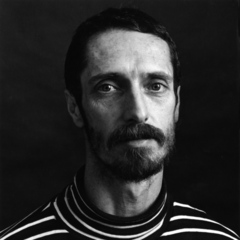
\includegraphics[width=0.25\textwidth]{images/history}
\end{wrapfigure}

\subsection{Founding Parents}\label{subsec:founding-parents}

CI was developed in June \textbf{1972} in the US by mainly \textbf{Steve Paxton} (``the father of CI'', see picture on the right), which was an American dancer, gymnastics and choreographer (and former Aikidoka, someone who practices the Japanese martial art Aikido) in New York City (Judson Dance Theater).
He wanted to explore and push the boundaries to develop this new practice, some sort of ``art-sport''.

Next to him, it is worth mentioning Nancy Stark Smith (``the mother of CI''), which is the one holding CI still, as Steve stopped doing CI about 7 years after the invention with the intention to giving it to the people.
She continued with another partner and started the Contact Quarterly magazine, a vehicle to share ideas, to hold the theme and practice of CI.

\subsection{Creational Event}\label{subsec:creational-event}

In spring 1972, Steve Paxton invited a group of 17 students and colleagues, dancers, martial artists, acrobats, gymnasts and athletes, to explore and research the \textbf{extremes of movement} and disorientation, from standing still to falling, rolling, colliding and jumping in the air, in a two-week workshop.
While moving with high velocity, running into each other, bumping, trying to survive, and see what the result will be.
A little like what they do in the Large Hadron Collider at CERN, smashing some particles at each other and be excited about what would happen.

He wanted the dancers to work with him on the form he was evolving, and at the end of this week of residency, the group presented a performance named \textbf{Contact Improvisations}.
To see for yourself how the first steps were made, have a look at this old recording: \url{https://www.youtube.com/watch?v=9FeSDsmIeHA}

Out of that exploration, a 20-minutes performance piece called ``\textit{Magnesium}'' arose, whereas the first quarter-hour was about jumping and bumping, manipulation and clinging.
Only the last 5 minutes the so-called ``\gls{smalldance}'' was performed: A form of meditation that is practiced standing, where attention is paid to postural adjustments and micro-weight transfers.
Videos narrated by Steve about that are available, which are very much encouraged to watch, to also see the progression from those impactful years of 72, 75 and 87.

\subsection{Organization}\label{subsec:organization}

At first, around 1975, it was considered to \textbf{trademark} the term contact improvisation, but this idea was rejected in favor of establishing a forum for communication, which nowadays is the online website \url{https://contactquarterly.com}, which is still co-edited by Nancy Stark Smith herself.
So the decision was very deliberate to not have any form of legal institute or certifications, free of any hierarchy.
A certificate usually doesn't mean that that person is good, but just that the certification was passed.

The downside of not having an authority verifying the competence of the teachers is of course that when the word was spreading, more and more injuries started to happen;
that's why one should never teach what one doesn't know properly.

\subsection{Further Spreading}\label{subsec:further-spreading}

A few years after the founding event, 1979, the very first ``Country Jam'' was organized, where 50 people came together to freely exchange and dance, without any structure.
Neither a workshop, conference nor seminar.
Co-created being, dancing and living in flux.
Later on it was introduced in new avant-garde dance schools in the US.

The members of the founding group scattered across the US and started to teach the practice.
It became smoother, continuous and controlled, yet still avoiding eye and direct hand contact.
Much emphasize was put on the experience of flow, which is more of an aesthetic choice (Nancy Stark Smith), yet the central characteristics preserved.

\textbf{Europe} was presented with CI first 1873 in Italy, and later Steve Paxton and Lisa Nelson regularly went to the UK and Amsterdam (School for New Dance Development) as the transmission belts for CI in the whole of Europe.
Belgium was visited by Paxton since the 1980s, but apart certain outbreaks of fever in successful jams, it didn't leave any lasting traces among dancers.

As founding people could be considered (next to Steve Paxton): Nancy Stark Smith, Danny Lepkoff, Lisa Nelson, Karen Nelson, Nita Little, Andrew Harwood, and Ray Chung.

For more detailed information read books like \textit{Sharing the Dance} and others which you can find in the ``\nameref{sec:resources}'' section.

\subsection{Then and Now}\label{subsec:then-and-now}

It was for sure very different back than, which is why also sometimes people would refer to it as ``old school contact'', which some are still doing.
There was a high risk with very high velocity, which for sure looked amazing -and scary.
Good to know though is, that they trained on mats, especially at the very beginning (see videos) which would make the impact of falling much less.
After they started to do the same with mats though, they got (quite a lot of) injuries.

The last few decades much more emphasizes was put on flow (instead on ``explosion''), and also figuring out the least resistant pathway.
Some people claim that CI lost quite a lot of its characteristic along the way, yet it could be said that it's nice to have both, to be able to choose what one wants.
Being able to survive the explosion, and play comfortably in the flow.

Today there are many styles: more flow, more impactful, acrobatics, dance, acting.
The differences are mostly based on the different teachers (lineages) but also due to culturally differences.
Different countries have simply different ``body orientations'', resulting in a different CI style.
